\begin{figure}[h!]
	\centering
	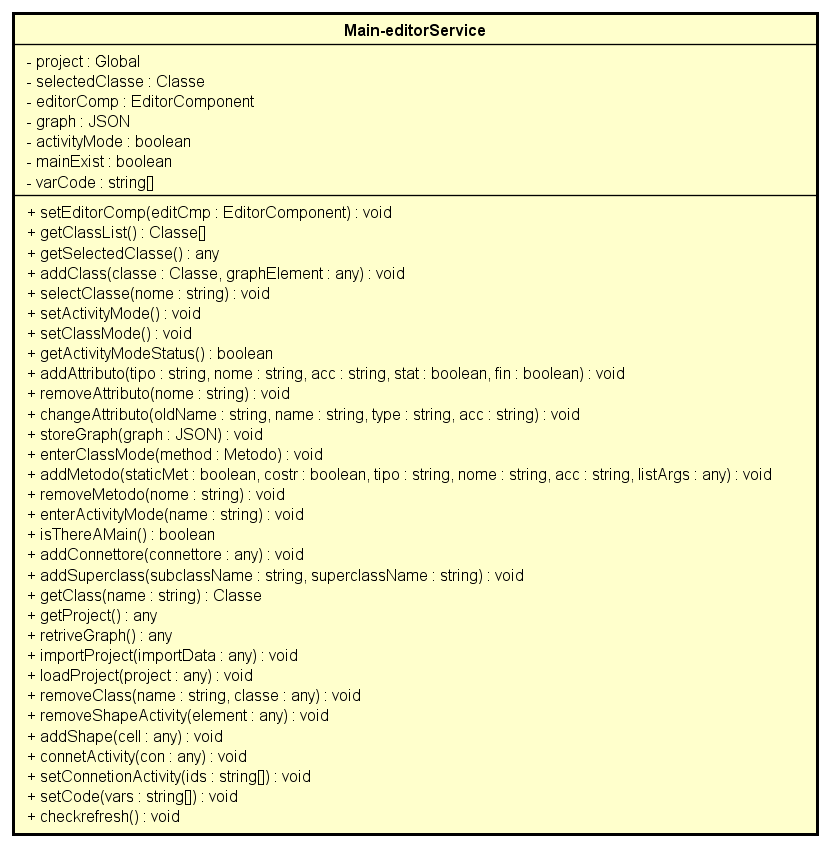
\includegraphics[scale=0.8]{res/sections/SpecificaFrontEnd/Services/Disegnetti/main-editor.png}
	\caption{Diagramma della classe Main-editorService}
\end{figure}

\begin{itemize}
	\item \textbf{Descrizione:}\\
	
	\item \textbf{Utilizzo:}\\
	
	\item \textbf{Attributi:}
		\begin{itemize}
			\item \emph{-project: Global}\\
			Serve per memorizzare informazioni riguardo il progetto corrente
			\item \emph{-selectedClasse: Classe}\\
			Memorizza la classe corrispondente nel canvas dell'editor
			\item \emph{-editorComp: EditorComponent}\\
			Serve per accedere direttamente all'EditorComponent
			\item \emph{-graph: JSON}\\
			Serve per memorizzare il grafico dell'editor
			\item \emph{-activityMode: boolean}\\
			Indica se è in uso l'activity diagram
			\item \emph{-mainExist: boolean}\\
			Indica se esiste il metodo main
			\item \emph{-varCode: string[]}\\
			
		\end{itemize}
	\item \textbf{Metodi:}
		\begin{itemize}
			\item \emph{+setEditorComp(editCmp: EditorComponent)}\\
    		Serve per costruire un istanziazione dell'EditorComponent\\
    		\textbf{Parametri:}
    		\begin{itemize}
    			\item \emph{editCmp: EditorComponent}\\
    			Istanzia EditorComponent
    		\end{itemize}
    		\item \emph{+getClassList()}\\
    		Ritorna la lista delle classi presenti nel progetto
    		\item \emph{+getSelectedClasse()}\\
    		Ritorna la classe selezionata
    		\item \emph{+addClass(classe: Classe, graphElement: any)}\\
    		Aggiunge un oggetto di tipo classe\\
    		\textbf{Parametri:}
    		\begin{itemize}
    			\item \emph{classe: Classe}\\
    			Classe da aggiungere
    			\item \emph{graphElement: any}\\
    			Elemento della libreria grafica
    		\end{itemize}
    		\item \emph{+selectClasse(nome: string)}\\
    		Cerca una classe all'interno della lista\\
    		\textbf{Parametri:}
    		\begin{itemize}
    			\item \emph{nome: string}\\
    			Nome della classe da cercare
    		\end{itemize}
    		\item \emph{+setActivityMode()}\\
    		Passa alla modalità activity diagram
    		\item \emph{+setClassMode()}\\
    		Passa alla modalità class diagram
    		\item \emph{+getActivityModeStatus()}\\
    		Ritorna il valore del fral activityMode
    		\item \emph{+addAttributo(tipo: string, nome:string, acc: string, stat: boolean, fin: boolean)}\\
    		Aggiunge un metodo alla selectedClasse\\
    		\textbf{Parametri:}
    		\begin{itemize}
    			\item \emph{tipo: string}\\
    			Tipo dell'attributo
    			\item \emph{nome:string}\\
    			Nome dell'attributo
    			\item \emph{acc: string}\\
    			Visibilità dell'attributo
    			\item \emph{stat: boolean}\\
    			True se è marcato static
    			\item \emph{fin: boolean}\\
    			True se è marcato final
    		\end{itemize}
    		\item \emph{+removeAttributo(nome: string)}\\
    		Rimuove un attributo dalla selectedClasse\\
    		\textbf{Parametri:}
    		\begin{itemize}
    			\item \emph{nome: string}\\
    			Nome dell'attributo da rimuovere
    		\end{itemize}
    		\item \emph{+changeAttributo(oldName: string, name: string, type: string, acc: string)}\\
    		Modifica un attributo della selectedClasse\\
    		\textbf{Parametri:}
    		\begin{itemize}
    			\item \emph{oldName: string}\\
    			Vecchio nome
    			\item \emph{name: string}\\
    			Nuovo nome
    			\item \emph{type: string}\\
    			Tipo dell'attributo
    			\item \emph{acc: string}\\
    			Visibilità dell'attributo
    		\end{itemize}
    		\item \emph{+storeGraph(graph: JSON)}\\
    		Memorizza il grafico\\
    		\textbf{Parametri:}
    		\begin{itemize}
    			\item \emph{graph: JSON}\\
    			Grafico da memorizzare
    		\end{itemize}
    		\item \emph{+enterClassMode(method: Metodo)}\\
    		Serve per ripristinare il diagramma delle classi dopo aver definito un metodo\\
    		\textbf{Parametri:}
    		\begin{itemize}
    			\item \emph{method: Metodo}\\
    			Metodo definito
    		\end{itemize}
    		\item \emph{+addMetodo(staticMet: boolean, costr: boolean, tipo: string, nome:string, acc: string, listArgs: any)}\\
    		Aggiunge un nuovo metodo alla selectedClasse\\
    		\textbf{Parametri:}
    		\begin{itemize}
    			\item \emph{staticMet: boolean}\\
    			True se è marcato static
    			\item \emph{costr: boolean}\\
    			True se è un costruttore
    			\item \emph{tipo: string}\\
    			Tipo di ritorno del metodo
    			\item \emph{nome:string}\\
    			Nome del metodo
    			\item \emph{acc: string}\\
    			Visibilità del metodo
    			\item \emph{listArgs: any}\\
    			Lista degli argomenti del metodo
    		\end{itemize}
    		\item \emph{+removeMetodo(nome: string)}\\
    		Rimuove un metodo dalla selectedClasse\\
    		\textbf{Parametri:}
    		\begin{itemize}
    			\item \emph{nome: string}\\
    			Nome del metodo da eliminare
    		\end{itemize}
    		\item \emph{+enterActivityMode(name: string)}\\
    		Entra nella modalità activity per modificare il corpo un metodo\\
    		\textbf{Parametri:}
    		\begin{itemize}
    			\item \emph{name: string}\\
    			Nome del metodo da modificare
    		\end{itemize}
    		\item \emph{+isThereAMain()}\\
    		Ritorna true se è presente il metodo main nella selectedClasse
    		\item \emph{+addConnettore(connettore: any)}\\
    		Aggiunge un connettore alla selectedClasse\\
    		\textbf{Parametri:}
    		\begin{itemize}
    			\item \emph{connettore: any}\\
    			Conettore da aggiungere
    		\end{itemize}
    		\item \emph{+addSuperclass(subclassName: string, superclassName: string)}\\
    		\\
    		\textbf{Parametri:}
    		\begin{itemize}
    			\item \emph{subclassName: string}\\
    			
    			\item \emph{superclassName: string}\\
    			
    		\end{itemize}
    		\item \emph{+getClass(name: string)}\\
    		\\
    		\textbf{Parametri:}
    		\begin{itemize}
    			\item \emph{name: string}\\
    			
    		\end{itemize}
    		\item \emph{+getProject()}\\
    		
    		\item \emph{+retriveGraph()}\\
    		
    		\item \emph{+importProject(importData: any)}\\
    		\\
    		\textbf{Parametri:}
    		\begin{itemize}
    			\item \emph{importData: any}\\
    			
    		\end{itemize}
    		\item \emph{+loadProject(project: any)}\\
    		\\
    		\textbf{Parametri:}
    		\begin{itemize}
    			\item \emph{project: any}\\
    			
    		\end{itemize}
    		\item \emph{+removeClass(name: string, classe: any)}\\
    		\\
    		\textbf{Parametri:}
    		\begin{itemize}
    			\item \emph{name: string}\\
    			
    			\item \emph{classe: any}\\
    			
    		\end{itemize}
    		\item \emph{+removeShapeActivity(element: any)}\\
    		\\
    		\textbf{Parametri:}
    		\begin{itemize}
    			\item \emph{element: any}\\
    			
    		\end{itemize}
    		\item \emph{addShape(cell: any)}\\
    		\\
    		\textbf{Parametri:}
    		\begin{itemize}
    			\item \emph{cell: any}\\
    			
    		\end{itemize}
    		\item \emph{+connetActivity(con: any)}\\
    		\\
    		\textbf{Parametri:}
    		\begin{itemize}
    			\item \emph{con: any}\\
    			
    		\end{itemize}
    		\item \emph{+setConnetionActivity(ids: string[])}\\
    		\\
    		\textbf{Parametri:}
    		\begin{itemize}
    			\item \emph{ids: string[]}\\
    			
    		\end{itemize}
    		\item \emph{+setCode(vars: string[])}\\
    		\\
    		\textbf{Parametri:}
    		\begin{itemize}
    			\item \emph{vars: string[]}\\
    			
    		\end{itemize}
    		\item \emph{+checkrefresh()}\\
    		
		\end{itemize}
\end{itemize}